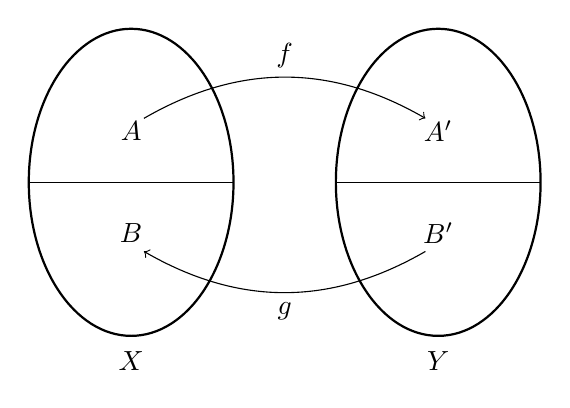
\begin{tikzpicture}[scale=0.65]
	% Sets X and Y
	\draw[thick] (0,0) ellipse (2 and 3);
	\draw[thick] (6,0) ellipse (2 and 3);

	% Labels for X and Y
	\node at (0,-3.5) {$X$};
	\node at (6,-3.5) {$Y$};

	% Subsets A and B in X
	\node at (0,1) {$A$};
	\node at (0,-1) {$B$};

	% Subsets A' and B' in Y
	\node at (6,1) {$A'$};
	\node at (6,-1) {$B'$};

	% Diagonal line between X and Y
	\draw (-2, 0) -- (2, 0);
	\draw (4, 0) -- (8, 0);

	\draw[-to, bend left] (0.25,1.25) to node[midway, above] {$f$} (5.75,1.25);
	\draw[-to, bend left] (5.75,-1.35) to node[midway, below] {$g$} (0.25,-1.35);
\end{tikzpicture}

